% !TEX root = ./Basilisk-pixelLineConverter-20190524.tex


\begin{figure}[H]
	\centerline{
		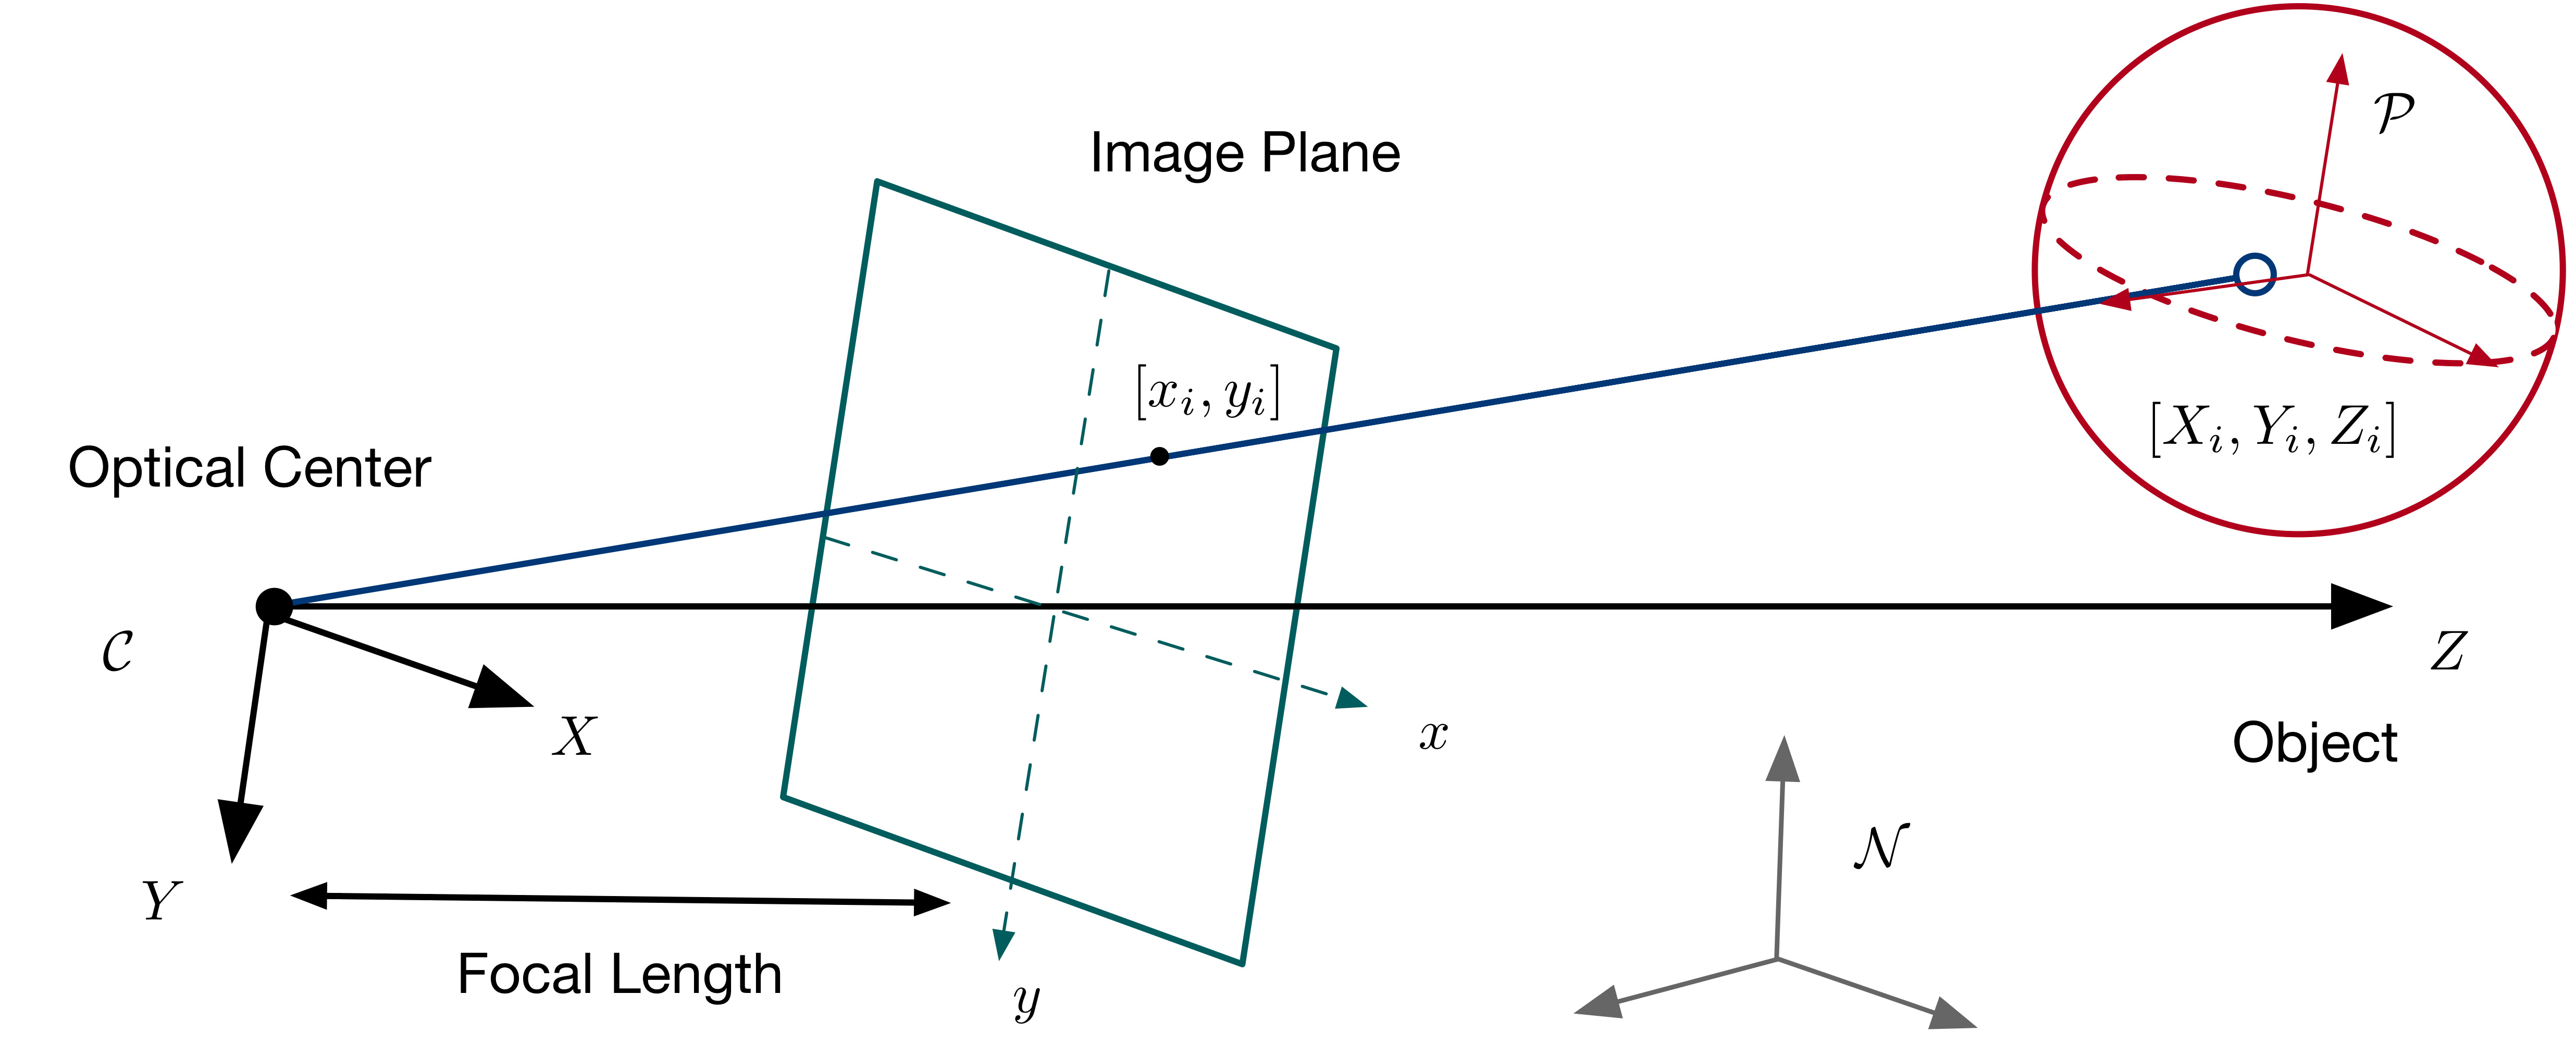
\includegraphics{Figures/CameraGeometry}
	}
	\caption{Camera Model}
	\label{fig:camera}
\end{figure}

\section{Model Description}

\subsection{Input and Output}

This converter module processes the output of a limb finding method to extract spacecraft inertial position. It does this by reading spacecraft attitude (coming from star tracker or other means), camera parameters, and the limb data. 

Messages read:

\begin{itemize}
\item CameraConfigMsgPayload: containing focal length, resolution, and sensor size. These values are needed for the following computations. Notably the camera frame relative to the body frame is used.
\item LimbInMsgPayload: Limb points, and uncertainty around these values in pixels. 
\item NavAttMsgPayload: Used for the spacecraft attitude. This allows to move from the body frame to the inertial frame.
\end{itemize}

Message written:
\begin{itemize}
\item OpNavMsgPayload: Message containing $\leftexp{N}{\bm r}$ and it's covariance.
\end{itemize}

\subsection{Position computation}

The details of the algorithm are summarized in the papers attached. The engineering note contains a summary of the algorithms and covariance analysis. The journal paper \cite{Chirstian_Limb} contains the details of the development and assumptions. 

The component that is chosen in the implementation is the way to solve the least squares for equation $$[H] \bm x = \bm 1$$

This is done in this module by performing a QR-decomposition via a a Gram-Schmidt process. This leads to the following equation:

$$[R] \bm x = [Q]^T\bm 1$$

Since $[R]$ is upper-triangular, this is solved with an implemented back-substitution. 